\documentclass[border=3pt,tikz]{standalone}
\usepackage{amsmath}
\usepackage{listofitems}
\usetikzlibrary{arrows.meta}
\usepackage[outline]{contour}
\contourlength{1.4pt}
\usetikzlibrary{fit,positioning}
\usepackage{xcolor}
\colorlet{myred}{red!80!black}
\colorlet{myblue}{blue!80!black}
\colorlet{mybluee}{myblue!80!black}
\colorlet{mygreen}{green!60!black}
\colorlet{myyellow}{yellow!88!black}
\colorlet{myorange}{orange!90!black}
\colorlet{mydarkred}{red!30!black}
\colorlet{mydarkblue}{blue!40!black}
\colorlet{mydarkgreen}{green!30!black}
\colorlet{mypurple}{violet!80!black}

\tikzset{
  >=latex,
  node/.style={thick,circle,draw=myblue,minimum size=22,inner sep=0.5,outer sep=0.6},
  node in/.style={node,green!20!black,draw=mygreen!30!black,fill=mygreen!25},
  node hidden/.style={node,blue!20!black,draw=myblue!30!black,fill=myblue!20},
  node out/.style={node,red!20!black,draw=myred!30!black,fill=myred!20},
  node mu/.style={node,yellow!20!black,draw=myyellow!30!black,fill=myyellow!20},
  node sigma/.style={node,orange!20!black,draw=myorange!30!black,fill=myorange!20},
  node sample/.style={node,purple!20!black,draw=mypurple!30!black,fill=mypurple!20},
  connect/.style={thick,mydarkblue},
}

\begin{document}
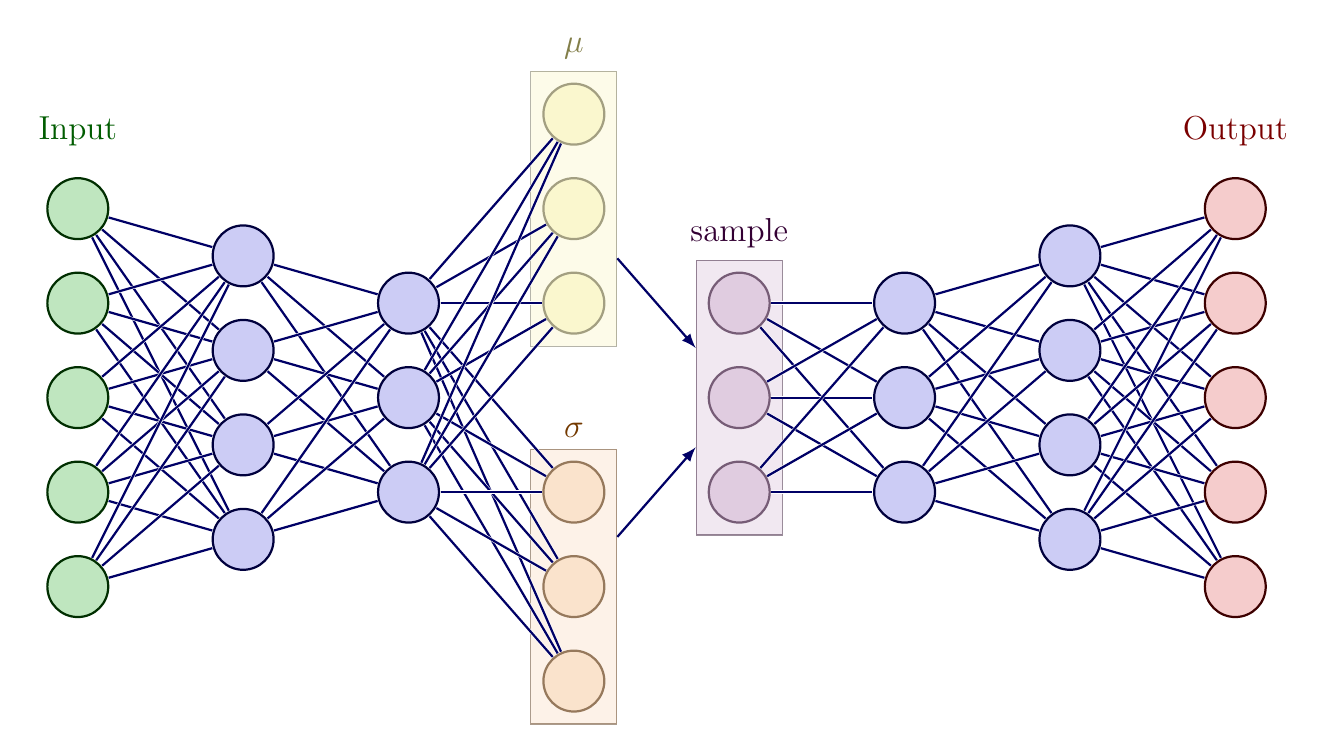
\begin{tikzpicture}[x=2.1cm,y=1.2cm]
  \large

  % Layer 1 (Input)
  \node[node in,outer sep=0.6] (N1-1) at (1,2) {};
  \node[node in,outer sep=0.6] (N1-2) at (1,1) {};
  \node[node in,outer sep=0.6] (N1-3) at (1,0) {};
  \node[node in,outer sep=0.6] (N1-4) at (1,-1) {};
  \node[node in,outer sep=0.6] (N1-5) at (1,-2) {};

  % Layer 2
  \node[node hidden,outer sep=0.6] (N2-1) at (2,1.5) {};
  \node[node hidden,outer sep=0.6] (N2-2) at (2,0.5) {};
  \node[node hidden,outer sep=0.6] (N2-3) at (2,-0.5) {};
  \node[node hidden,outer sep=0.6] (N2-4) at (2,-1.5) {};

  % Layer 3
  \node[node hidden,outer sep=0.6] (N3-1) at (3,1) {};
  \node[node hidden,outer sep=0.6] (N3-2) at (3,0) {};
  \node[node hidden,outer sep=0.6] (N3-3) at (3,-1) {};

  % Layer 4
  \node[node mu,outer sep=0.6] (N4-1) at (4,3) {};
  \node[node mu,outer sep=0.6] (N4-2) at (4,2) {};
  \node[node mu,outer sep=0.6] (N4-3) at (4,1) {};
  \node[node sigma,outer sep=0.6] (N4-4) at (4,-1) {};
  \node[node sigma,outer sep=0.6] (N4-5) at (4,-2) {};
  \node[node sigma,outer sep=0.6] (N4-6) at (4,-3) {};
  \node [label=\textcolor{myyellow!50!black}{$\mu$}, fit=(N4-1)(N4-3), yellow!20!black,draw=myyellow!30!black,fill=myyellow!20, opacity=0.45] (mu) {};
  \node [label=\textcolor{myorange!50!black}{$\sigma$}, fit=(N4-4)(N4-6), orange!20!black,draw=myorange!30!black,fill=myorange!20, opacity=0.45] (sigma) {};

  % Layer 5
  \node[node sample,outer sep=0.6] (N5-1) at (5,1) {};
  \node[node sample,outer sep=0.6] (N5-2) at (5,0) {};
  \node[node sample,outer sep=0.6] (N5-3) at (5,-1) {};
  \node [label=\textcolor{mypurple!50!black}{sample}, fit=(N5-1)(N5-3), purple!20!black,draw=mypurple!30!black,fill=mypurple!20, opacity=0.45] (sample) {};
  
  % Layer 6
  \node[node hidden,outer sep=0.6] (N6-1) at (6,1) {};
  \node[node hidden,outer sep=0.6] (N6-2) at (6,0) {};
  \node[node hidden,outer sep=0.6] (N6-3) at (6,-1) {};

  % Layer 7
  \node[node hidden,outer sep=0.6] (N7-1) at (7,1.5) {};
  \node[node hidden,outer sep=0.6] (N7-2) at (7,0.5) {};
  \node[node hidden,outer sep=0.6] (N7-3) at (7,-0.5) {};
  \node[node hidden,outer sep=0.6] (N7-4) at (7,-1.5) {};

  % Layer 8 (Output)
  \node[node out,outer sep=0.6] (N8-1) at (8,2) {};
  \node[node out,outer sep=0.6] (N8-2) at (8,1) {};
  \node[node out,outer sep=0.6] (N8-3) at (8,0) {};
  \node[node out,outer sep=0.6] (N8-4) at (8,-1) {};
  \node[node out,outer sep=0.6] (N8-5) at (8,-2) {};

  % Connections (Layer 1 to 2)
  \foreach \i in {1,...,5}
    \foreach \j in {1,...,4} {
      \draw[connect,white,line width=1.2] (N1-\i) -- (N2-\j);
      \draw[connect] (N1-\i) -- (N2-\j);
    }

  % Connections (Layer 2 to 3)
  \foreach \i in {1,...,4}
    \foreach \j in {1,...,3} {
      \draw[connect,white,line width=1.2] (N2-\i) -- (N3-\j);
      \draw[connect] (N2-\i) -- (N3-\j);
    }

  % Connections (Layer 3 to 4)
  \foreach \i in {1,...,3}
    \foreach \j in {1,...,6} {
      \draw[connect,white,line width=1.2] (N3-\i) -- (N4-\j);
      \draw[connect] (N3-\i) -- (N4-\j);
    }

  % % Connections (Layer 4 to 5)
  % \foreach \i in {1,...,6}
  %   \foreach \j in {1,...,3} {
  %     \draw[connect,white,line width=1.2] (N4-\i) -- (N5-\j);
  %     \draw[connect] (N4-\i) -- (N5-\j);
  %   }

  % Connections (Layer 5 to 6)
  \foreach \i in {1,...,3}
    \foreach \j in {1,...,3} {
      \draw[connect,white,line width=1.2] (N5-\i) -- (N6-\j);
      \draw[connect] (N5-\i) -- (N6-\j);
    }

  % Connections (Layer 6 to 7)
  \foreach \i in {1,...,3}
    \foreach \j in {1,...,4} {
      \draw[connect,white,line width=1.2] (N6-\i) -- (N7-\j);
      \draw[connect] (N6-\i) -- (N7-\j);
    }

  % Connections (Layer 7 to 8)
  \foreach \i in {1,...,4}
    \foreach \j in {1,...,5} {
      \draw[connect,white,line width=1.2] (N7-\i) -- (N8-\j);
      \draw[connect] (N7-\i) -- (N8-\j);
    }

   \draw[connect, ->] (mu) -- (sample);
   \draw[connect, ->] (sigma) -- (sample);

  % Labels
  \node[above=0.2,align=center,mygreen!60!black] at (N1-1.90) {Input};
  \node[above=0.2,align=center,myred!60!black] at (N8-1.90) {Output};

\end{tikzpicture}
\end{document}







% Variational autoencoder architecture. The earliest type of generative machine learning model.
% Inspired by https://towardsdatascience.com/intuitively-understanding-variational-autoencoders-1bfe67eb5daf.

\documentclass[tikz]{standalone}

\usepackage{xstring}

% COLORS
\usepackage{xcolor}
\colorlet{myred}{red!80!black}
\colorlet{myblue}{blue!80!black}
\colorlet{mygreen}{green!60!black}
\colorlet{myorange}{orange!70!red!60!black}
\colorlet{mydarkred}{red!30!black}
\colorlet{mydarkblue}{blue!40!black}
\colorlet{mydarkgreen}{green!30!black}

% STYLES
\tikzset{
  >=latex, % for default LaTeX arrow head
  node/.style={thick,circle,draw=myblue,minimum size=22,inner sep=0.5,outer sep=0.6},
  node in/.style={node,green!20!black,draw=mygreen!30!black,fill=mygreen!25},
  node hidden/.style={node,blue!20!black,draw=myblue!30!black,fill=myblue!20},
  node convol/.style={node,orange!20!black,draw=myorange!30!black,fill=myorange!20},
  node out/.style={node,red!20!black,draw=myred!30!black,fill=myred!20},
  connect/.style={thick,mydarkblue}, %,line cap=round
  connect arrow/.style={-{Latex[length=4,width=3.5]},thick,mydarkblue,shorten <=0.5,shorten >=1},
  node 1/.style={node in}, % node styles, numbered for easy mapping with \nstyle
  node 2/.style={node hidden},
  node 3/.style={node out}
}


\usetikzlibrary{fit,positioning}

\newcommand\drawNodes[2]{
  % #1 (str): namespace
  % #2 (list[list[str]]): list of labels to print in the node of each neuron
  \foreach \neurons [count=\lyrIdx] in #2 {
    \StrCount{\neurons}{,}[\lyrLength] % use xstring package to save each layer size into \lyrLength macro
    \foreach \n [count=\nIdx] in \neurons
      \node[neuron] (#1-\lyrIdx-\nIdx) at (2*\lyrIdx, \lyrLength/2-1.4*\nIdx) {\n};
  }
}

\newcommand\denselyConnectNodes[2]{
  % #1 (str): namespace
  % #2 (list[int]): number of nodes in each layer
  \foreach \n [count=\lyrIdx, remember=\lyrIdx as \previdx, remember=\n as \prevn] in #2 {
    \foreach \y in {1,...,\n} {
      \ifnum \lyrIdx > 1
        \foreach \x in {1,...,\prevn}
          \draw[connect] (#1-\previdx-\x) -- (#1-\lyrIdx-\y);
      \fi
    }
  }
}

\begin{document}
\begin{tikzpicture}[
    shorten >=1pt, shorten <=1pt,
    neuron/.style={circle, draw, minimum size=4ex, thick},
    legend/.style={font=\large\bfseries},
  ]

  % encoder
  \drawNodes{encoder}{{{,,,,}, {,,,}, {,,}}}
  \denselyConnectNodes{encoder}{{5, 4, 3}}

  % decoder
  \begin{scope}[xshift=11cm]
    \drawNodes{decoder}{{{,,}, {,,,}, {,,,,}}}
    \denselyConnectNodes{decoder}{{3, 4, 5}}
  \end{scope}

  % mu, sigma, sample nodes
  \foreach \idx in {1,...,3} {
      \coordinate[neuron, right=2 of encoder-3-2, yshift=\idx cm,, fill=yellow, fill opacity=0.2] (mu-\idx);
      \coordinate[neuron, right=2 of encoder-3-2, yshift=-\idx cm, fill=blue, fill opacity=0.1] (sigma-\idx);
      \coordinate[neuron, right=4 of encoder-3-2, yshift=\idx cm-2cm, fill=green, fill opacity=0.1] (sample-\idx);
    }

  % mu, sigma, sample boxes
  \node [label=$\mu$, fit=(mu-1) (mu-3), draw, fill=yellow, opacity=0.45] (mu) {};
  \node [label=$\sigma$, fit=(sigma-1) (sigma-3), draw, fill=blue, opacity=0.3] (sigma) {};
  \node [label=sample, fit=(sample-1) (sample-3), draw, fill=green, opacity=0.3] (sample) {};

  % mu, sigma, sample connections
  \draw[connect] (mu.east) edge (sample.west) (sigma.east) -- (sample.west);
  \foreach \a in {1,2,3}
  \foreach \b in {1,2,3} {
      \draw[connect] (encoder-3-\a) -- (mu-\b);
      \draw[connect] (encoder-3-\a) -- (sigma-\b);
      \draw[connect] (sample-\a) -- (decoder-1-\b);
    }


  \node[above=0.1 of encoder-1-1] {Input};
  \node[above=0.1 of decoder-3-1] {Output};

\end{tikzpicture}
\end{document}


